% Created 2021-10-09 Sat 15:47
% Intended LaTeX compiler: pdflatex
\documentclass[a4paper, 11pt, twoside]{article}
\usepackage[utf8]{inputenc}
\usepackage[T1]{fontenc}
\usepackage{graphicx}
\usepackage{grffile}
\usepackage{longtable}
\usepackage{wrapfig}
\usepackage{rotating}
\usepackage[normalem]{ulem}
\usepackage{amsmath}
\usepackage{textcomp}
\usepackage{amssymb}
\usepackage{capt-of}
\usepackage{hyperref}
\usepackage{baskervillef}
\usepackage{geometry}\geometry{ a4paper, total={170mm,257mm}, left=20mm, top=20mm,}
\usepackage{hyperref}\hypersetup{pdfauthor={Olivier Rey}, pdftitle={Dungeon Squad! - Version Française}, pdfkeywords={jdr, dungeonsquad}, pdfsubject={jeu de rôles}, pdfcreator={Emacs 26.1 (Org mode 9.1.9)}, pdflang={Frenchb}, colorlinks=true, linkcolor={blue}, urlcolor={blue}}
\usepackage[french, frenchb]{babel}
\usepackage{titlesec}\titlelabel{\thetitle. \quad}
\usepackage[table,svgnames]{xcolor}\rowcolors{1}{Gainsboro}{WhiteSmoke}
\usepackage{etoolbox}\AtBeginEnvironment{longtable}{\small}
\author{Olivier Rey}
\date{2021-10-09}
\title{Générateur de labyrinthes pour JDR}
\hypersetup{
 pdfauthor={Olivier Rey},
 pdftitle={Générateur de labyrinthes pour JDR},
 pdfkeywords={},
 pdfsubject={},
 pdfcreator={Emacs 26.1 (Org mode 9.1.9)}, 
 pdflang={Frenchb}}
\begin{document}

\maketitle
\tableofcontents

\newpage

\section{Générateur de labyrinthes pour JDR}
\label{sec:orgcc9f3fe}

\subsection{Introduction}
\label{sec:org700493e}

John Norio a travaillé sur plusieurs versions de générateurs de "donjons", ce qui est traduit par générateur de labyrinthe. Nous proposons ici la traduction de la version 4.1 du générateur.

\begin{longtable}{ll}
Concepteur & (C) John Yorio "No Budget No Frills Pencil and Paper Dungeon Generator"\\
Version & 4.1\\
URL & \href{http://tabletopdiversions.blogspot.com/2012/12/dungeon-generator-updated-now-with-more.html}{http://tabletopdiversions.blogspot.com/}\\
Traduction et adaptation & (C) O. Rey avril 2021\\
Version 1.1 & Adaptation PDF\\
\end{longtable}

\subsection{Matériel}
\label{sec:orgc648b18}

\begin{itemize}
\item Un jeu de cartes ordinaire de 54 cartes sans les jokers.
\item Des dés : 1D4, 1D6, 1D8, 1D10.
\item Du papier quadrillé, des crayons ou stylos ou un équivalent informatique.
\end{itemize}

\subsection{Enchaînement des tables}
\label{sec:org4f27e1a}

\begin{center}
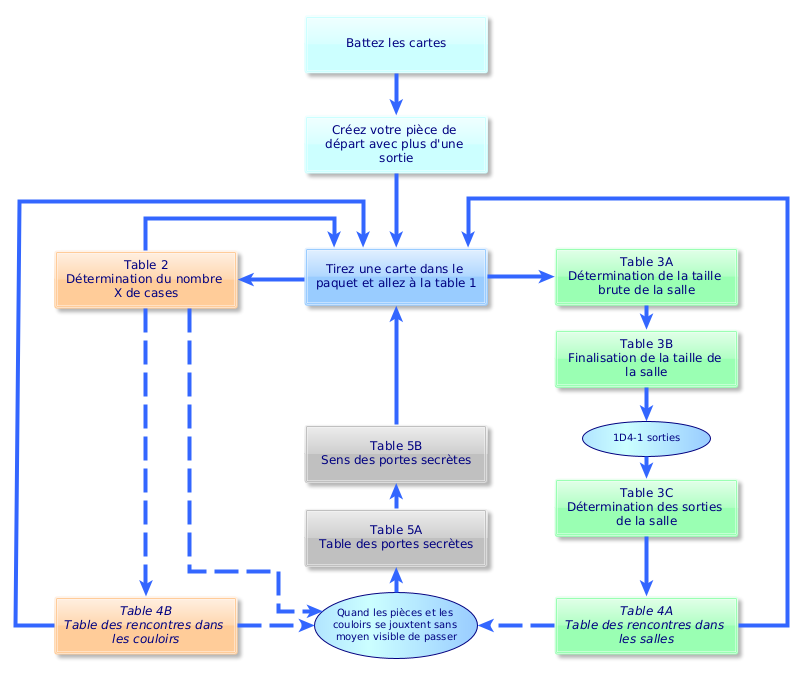
\includegraphics[width=.9\linewidth]{genlab01.png}
\end{center}

Gardez en mémoire que vous pouvez toujours adapter un peu les choses si votre labyrinthe ne rentre pas dans la page.

\newpage

\section{Tables}
\label{sec:org2fe85e1}

\subsection{Table principale}
\label{sec:org7b4eea3}

\begin{longtable}{cp{6cm}p{8.5cm}}
\emph{Table 1} & \emph{Table principale} & \\
\textbf{Carte} & \textbf{Résultat} & \textbf{Détails}\\
As & Escaliers montants, ou sortie dans X cases & Choix du joueur ou lancer 1D6 : 1-3 escaliers, 4-6 sortie\\
2 & Escaliers descendants, ou sortie dans X cases & Choix du joueur ou lancer 1D6 : 1-3 escaliers, 4-6 sortie\\
3 & Couloir droit pendant X cases avec piège & Lancer 1D6 : 1-3 fosse, 4-6 autre piège\\
4 & Couloir droit pendant X cases & \\
5 & Intersection en croix dans X cases & Couloirs à gauche, à droite et devant\\
6 & Coude à droite dans X cases & \\
7 & Coude à gauche dans X cases & \\
8 & Intersection en T dans X cases & Lancer 1D6 : 1-2 coudes à gauche et à droite, 3-4 coude à gauche et couloir devant, 5-6 coude à droite et couloir devant\\
9-10-Valet & \textbf{Salle} & Dessiner une porte et aller aux tables 3A, puis 3B, puis 3C\\
Dame & Impasse dans X cases, ou tirer une autre carte & Choix du joueur\\
Roi & Rebattez les cartes et tirez une nouvelle carte & Variante : gardez le roi de côté et tirez une nouvelle carte. Au quatrième roi, rebattez les cartes et tirez un nouvelle carte\\
\end{longtable}


\subsection{Couloirs}
\label{sec:org8a56d54}

\begin{longtable}{cc}
\emph{Table 2} & \emph{Détermination du nombre X de cases}\\
\textbf{Couleur de la carte} & \textbf{Nombre de cases}\\
Coeur & 1D10\\
Carreau & 1D8\\
Pique & 1D6\\
Trèfle & 1D4\\
\end{longtable}


\begin{longtable}{cl}
\emph{Table 4B} & \emph{Table des rencontres dans les couloirs (optionnel)}\\
\textbf{1D6} & \textbf{Rencontre}\\
1 & Monstre\\
2 & Piège\\
3-6 & Rien à signaler\\
\end{longtable}

Vous pouvez aussi utiliser les tables de rencontres de votre jeu favori.

\subsection{Salles}
\label{sec:org4ac4021}

\begin{longtable}{cc}
\emph{Table 3A} & \emph{Taille brute de la salle}\\
\textbf{Couleur de la carte} & \textbf{Nombre de cases}\\
Coeur & D10 x D10 cases\\
Carreaux & D8 x D8 cases\\
Pique & D6 x D6 cases\\
Trèfle & D4 x D4 cases\\
\end{longtable}


\begin{longtable}{cl}
\emph{Table 3B} & \emph{Finalisation de la taille de la salle}\\
\textbf{Analyse des dés} & \textbf{Action}\\
Les deux dés ont la même valeur & Pas de changement\\
Un dé est pair et l'autre impair & Diviser le plus grand nombre en deux et arrondir au chiffre supérieur\\
Si les deux dés sont pairs ou impairs & Diviser les deux nombres par deux et arrondir au chiffre supérieur\\
\end{longtable}


\begin{longtable}{cl}
\emph{Table 3C} & \emph{Détermination des 1D4-1 sorties}\\
\textbf{1D6} & \textbf{Positionnement de la sortie}\\
1-2 & Sortie à gauche de la porte d'entrée\\
3-4 & Sorie en face de la porte d'entrée\\
5-6 & Sortie à droite de la porte d'entrée\\
\end{longtable}


\begin{longtable}{cl}
\emph{Table 4A} & \emph{Table des rencontres dans les salles}\\
\textbf{1D6} & \textbf{Rencontre}\\
1-2 & Monstre\\
3 & Piège\\
4 & Situation étrange (statues qui parlent, fontaine magique, etc.)\\
5-6 & Vide\\
\end{longtable}

\subsection{Portes secrètes}
\label{sec:org1578121}

Qund les pièces et les couloirs se jouxtent sans moyen visible de passer, il se peut qu'il y ait une porte secrète.

\begin{longtable}{cl}
\emph{Table 5A} & \emph{Portes secrètes}\\
\textbf{1D6} & \textbf{A trouver}\\
1 & Porte secrète\\
2-6 & Rien\\
\end{longtable}


\begin{longtable}{cl}
\emph{Table 5B} & \emph{Sens des portes secrètes}\\
\textbf{1D6} & \textbf{Sens}\\
1 & Sens unique dans la direction dans laquelle vous allez\\
2-5 & Double sens\\
6 & Sens unique dans la direction opposée à celle dans laquelle vous allez\\
\end{longtable}


\vfill

\begin{center}

\includegraphics[width=3cm]{logo-orey-big.png}
\end{center}
\end{document}
